\section{Reverberation Chamber}
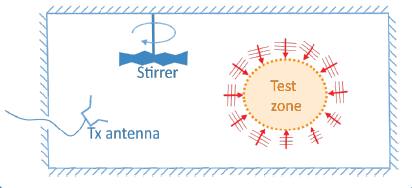
\includegraphics[width=8cm]{content/at_meas/pictures/reverberation_chamber}

A test chamber, contain ig a highly unsymmetric stirrer, designed to generate a \textbf{stochastical field distribution} in the test zone.

Ideally, it should have:
\begin{itemize}
  \item Electrically large cavity resonator with high $Q$ factor,
  \item High field strength for moderate input power,
  \item At least 60 resonant mode (IEEE 149--2022).
\end{itemize}

\subsection{Test Zone}
The ideal test zone field is:
\begin{itemize}
  \item isotropic (no preferred incident angle),
  \item homogenous (same magnitude everywhere),
  \item and unpolarized.
\end{itemize}

It can be described by a plane wave expansion:
\begin{equation}
  \bs{E}(\bs{r}) \oiint\limits_{\Omega} \bs{F}(\hat{\bs{k}}) \, e^{-j\bs{k}\cdot\bs{r}}\, \mathrm{d}^{2}\hat{\bs{k}}.
\end{equation}

 \todo{chamber statistics}
